\documentclass[a4paper]{article}\usepackage[]{graphicx}\usepackage[]{color}
% maxwidth is the original width if it is less than linewidth
% otherwise use linewidth (to make sure the graphics do not exceed the margin)
\makeatletter
\def\maxwidth{ %
  \ifdim\Gin@nat@width>\linewidth
    \linewidth
  \else
    \Gin@nat@width
  \fi
}
\makeatother

\definecolor{fgcolor}{rgb}{0.345, 0.345, 0.345}
\newcommand{\hlnum}[1]{\textcolor[rgb]{0.686,0.059,0.569}{#1}}%
\newcommand{\hlstr}[1]{\textcolor[rgb]{0.192,0.494,0.8}{#1}}%
\newcommand{\hlcom}[1]{\textcolor[rgb]{0.678,0.584,0.686}{\textit{#1}}}%
\newcommand{\hlopt}[1]{\textcolor[rgb]{0,0,0}{#1}}%
\newcommand{\hlstd}[1]{\textcolor[rgb]{0.345,0.345,0.345}{#1}}%
\newcommand{\hlkwa}[1]{\textcolor[rgb]{0.161,0.373,0.58}{\textbf{#1}}}%
\newcommand{\hlkwb}[1]{\textcolor[rgb]{0.69,0.353,0.396}{#1}}%
\newcommand{\hlkwc}[1]{\textcolor[rgb]{0.333,0.667,0.333}{#1}}%
\newcommand{\hlkwd}[1]{\textcolor[rgb]{0.737,0.353,0.396}{\textbf{#1}}}%
\let\hlipl\hlkwb

\usepackage{framed}
\makeatletter
\newenvironment{kframe}{%
 \def\at@end@of@kframe{}%
 \ifinner\ifhmode%
  \def\at@end@of@kframe{\end{minipage}}%
  \begin{minipage}{\columnwidth}%
 \fi\fi%
 \def\FrameCommand##1{\hskip\@totalleftmargin \hskip-\fboxsep
 \colorbox{shadecolor}{##1}\hskip-\fboxsep
     % There is no \\@totalrightmargin, so:
     \hskip-\linewidth \hskip-\@totalleftmargin \hskip\columnwidth}%
 \MakeFramed {\advance\hsize-\width
   \@totalleftmargin\z@ \linewidth\hsize
   \@setminipage}}%
 {\par\unskip\endMakeFramed%
 \at@end@of@kframe}
\makeatother

\definecolor{shadecolor}{rgb}{.97, .97, .97}
\definecolor{messagecolor}{rgb}{0, 0, 0}
\definecolor{warningcolor}{rgb}{1, 0, 1}
\definecolor{errorcolor}{rgb}{1, 0, 0}
\newenvironment{knitrout}{}{} % an empty environment to be redefined in TeX

\usepackage{alltt}
\usepackage[left=2.5cm,top=3cm,bottom=3.5cm,right=2.5cm]{geometry} % Ajustar Margenes
\usepackage[spanish, es-tabla, es-nodecimaldot]{babel} % para producir la letras acentuadas "?"
\usepackage[utf8]{inputenc} % ecribir acentos ?
\usepackage{booktabs} % Para crear tablas
\usepackage{graphicx} % Para manipular imagenes 
\usepackage{amsmath} % Para el manejo de ecuaciones
\usepackage{color} % Para los colores
\usepackage{hyperref}
\hypersetup{colorlinks=true, linkcolor=blue, filecolor=magenta, urlcolor=blue}
\title{Resultados} % Agregar titulo
\author{Rafael Eduardo Diaz} % Agregar Nombre

\setlength{\abovecaptionskip}{2pt plus 1pt minus 0pt} % Chosen fairly arbitrarily



\IfFileExists{upquote.sty}{\usepackage{upquote}}{}
\begin{document}

\maketitle
\section{Aplicación e ilustración}

A continuación, ilustramos todos los modelos descritos anteriormente aplicándolos a dos conjuntos de datos, para la serie anual del número de homicidios en Colombia de 1960 a 2018 se ajustaron varios PHMM, mientras que para la serie mensual de incendios forestales en Colombia, entre el 2002 y 2016 se ajustaron diversos ZIP-HMM. Antes de que se ajusten los modelos, se llevo a cabo un análisis exploratorio básico del conjunto de datos que aborda algunos problemas que generalmente se presentan al visualizar los datos de conteo. Al final de la sección, se comparan todos los modelos ajustados, tanto desde el enfoque clásico como Bayesiano, y se selecciona el mejor modelo a partir de las dos metodologías. 

\vspace{5mm} %5mm vertical space

Para ambas series, la aplicación de modelos estándar como modelos auto regresivos de media móvil (ARMA) sería inapropiado, ya que estos modelos se basan en la distribución normal. En cambio, se propone un modelo usual para datos con conteos la distribución de Poisson, pero, como se demostrará más adelante, las series presenta una sobredispersión considerable con respecto a la distribución de Poisson, y fuerte dependencia serial positiva además de inflación en ceros en el caso de la serie de incendios. Por lo tanto, un modelo que consiste en variables aleatorias independientes de Poisson; sería por dos razones inadecuado. Primero que puede haber algunos períodos con una baja tasa de homicidios e incendios, y algunos con una tasa relativamente alta. Los HMMs, permiten que la distribución de probabilidad de cada observación dependa del estado no observado (u oculto) de una cadena de Markov, por lo tanto puede acomodar la sobredispersión y la dependencia serial al mismo tiempo.



\subsection{Descripción de los datos}

\textbf{Homicidios:} Esta tabla contiene las cifras actualizadas de homicidios en Colombia 1960-2018, con base en la Compilación de estadísticas históricas económicas y sociales, extraída del \href{https://www.dnp.gov.co/estudios-y-publicaciones/estudios-economicos/Paginas/estadisticas-historicas-de-colombia.aspx}{departamento Nacional de Planeación} (DNP) se consulto específicamente el capítulo 8 indicadores de violencia, se complemento junto con las estadísticas delectivas de la \href{https://www.policia.gov.co/grupo-información-criminalidad/estadistica-delictiva}{Policía Nacional} y Medicina Legal. Los datos publicados corresponden a consolidados de los Delitos de Impacto del país, así mismo la Actividad Operativa realizada por la Policía Nacional. Mientras que para la población total Colombiana se extrajo la información de la sección Estadísticas por tema, demografía y población. La serie es anual para un total de 59 observaciones y se expresa como el número de homicidios por cada 100.000 habitantes comunmente conocida como \emph{Tasa de homicidios}, para ser posible la modelación se redondeo la cifra al entero más cercano. Nota: La confiabilidad de los datos de la tasa de asesinatos puede variar, de acuerdo a la fuente.

% latex table generated in R 3.4.4 by xtable 1.8-4 package
% Fri Jun 21 20:26:55 2019
\begin{table}[ht]
\centering
\begin{tabular}{rrrrrrrrrrrrrrrrrrrr}
  \hline
  \hline
31 & 31 & 31 & 32 & 31 & 32 & 30 & 29 & 31 & 19 & 21 & 23 & 23 & 23 & 24 & 24 & 25 & 27 & 26 & 27 \\ 
  29 & 36 & 34 & 30 & 30 & 40 & 48 & 52 & 63 & 65 & 68 & 78 & 76 & 74 & 70 & 66 & 68 & 62 & 58 & 61 \\ 
  65 & 49 & 69 & 56 & 48 & 42 & 40 & 39 & 36 & 35 & 34 & 32 & 32 & 32 & 27 & 26 & 25 & 25 & 25 &  \\ 
   \hline
\end{tabular}
\caption{Número de homicidios por 100.000 habitantes en Colombia, 1960 - 2018.} 
\end{table}


\vspace{5mm} %5mm vertical space

\textbf{Incendios:} Los datos referentes a incendios forestales en Colombia, fueron recolectados de la página del IDEAM - Instituto de Hidrología, Meteorología y Estudios Ambientales que ha venido realizando una revisión histórica y consolidado de los datos reportados por las siguientes instituciones: entidades del SINA, entidades del Sistema Nacional para la Prevención y atención de Desastres, la Defensa Civil, entre otras, y aunque se ha adoptado un Formulario Único de Captura (MAVDT \& otros, 2002), con el fin de estandarizar la información, este no ha sido utilizado en su totalidad y existen otros formatos desarrollados por las distintas entidades, de acuerdo con sus particularidades técnicas e informáticas, lo que ha dificultado la estandarización en el flujo de información.
\\
Las estadísticas sobre incendios en Colombia, permiten en términos generales, realizar análisis de su comportamiento bajo diferentes escenarios, esto es, por regiones, departamentos o municipios, con Niño o en condiciones climáticas normales,  por cobertura vegetal afectada, por Corporación Autónoma Regional, por año o por mes, y de esta manera, poder ser  utilizarlas para priorizar áreas, orientar acciones o sustentar la necesidad de realizar estudios más detallados. El Ideam ha venido realizando una revisión histórica de los datos reportados por las instituciones anteriormente mencionadas, con el fin de tener datos más confiables que permitan tener una mejor aproximación al tema. La variable de interés es el número de grandes incendios forestales (GIF), y se definen como aquellos incendios que superan las 500 hectáreas forestales afectadas. El número de observaciones es mensual iniciando en enero del 2002 y finalizando en diciembre del 2016, para un total 180 observaciones.

[1] ".preformat.ts"
% latex table generated in R 3.4.4 by xtable 1.8-4 package
% Fri Jun 21 20:26:55 2019
\begin{table}[ht]
\centering
\begin{tabular}{rrrrrrrrrrrrr}
  \hline
 & Jan & Feb & Mar & Apr & May & Jun & Jul & Aug & Sep & Oct & Nov & Dec \\ 
  \hline
2002 &   0 &   1 &   4 &   0 &   0 &   0 &   0 &   0 &   0 &   0 &   0 &   0 \\ 
  2003 &   0 &   2 &   1 &   0 &   0 &   0 &   0 &   0 &   0 &   0 &   0 &   0 \\ 
  2004 &   1 &   6 &   3 &   0 &   0 &   0 &   0 &   1 &   0 &   0 &   0 &   0 \\ 
  2005 &   0 &   0 &   1 &   0 &   0 &   0 &   0 &   1 &   2 &   0 &   0 &   0 \\ 
  2006 &   0 &   0 &   0 &   0 &   0 &   0 &   2 &   0 &   0 &   0 &   0 &   0 \\ 
  2007 &   3 &  23 &   3 &   0 &   0 &   0 &   0 &   0 &   0 &   0 &   0 &   0 \\ 
  2008 &   0 &   1 &   1 &   0 &   0 &   0 &   0 &   0 &   0 &   0 &   0 &   0 \\ 
  2009 &   0 &   0 &   0 &   0 &   0 &   0 &   1 &   2 &   2 &   1 &   0 &   1 \\ 
  2010 &  20 &  16 &   6 &   0 &   0 &   0 &   0 &   0 &   0 &   0 &   0 &   0 \\ 
  2011 &   1 &  10 &   0 &   0 &   0 &   0 &   0 &   0 &   0 &   0 &   0 &   0 \\ 
  2012 &   1 &   3 &   3 &   0 &   0 &   0 &   2 &   1 &   8 &   0 &   0 &   0 \\ 
  2013 &   4 &   6 &   2 &   0 &   0 &   0 &   0 &   1 &   3 &   0 &   0 &   0 \\ 
  2014 &   4 &   4 &  11 &   4 &   0 &   0 &   5 &   4 &   3 &   0 &   0 &   0 \\ 
  2015 &   1 &   2 &   3 &   1 &   0 &   0 &   0 &   6 &   6 &   0 &   0 &   0 \\ 
  2016 &   1 &  10 &  18 &   0 &   0 &   0 &   0 &   2 &   1 &   0 &   0 &   0 \\ 
   \hline
\end{tabular}
\caption{Número de Grandes Incendios Forestales (GIF) en Colombia, 2002 - 2016.} 
\end{table}


\subsubsection*{Estadísticas de resumen}

A continuación se muestran algunas estadísticas descriptivas, sobre la serie de homicidios Colombia para los años 1960-2018.


\begin{table}[!htbp] \centering 
  \caption{Estadísticas de Resumen serie homicidios en Colombia.} 
  \label{} 
\begin{tabular}{@{\extracolsep{5pt}}lcccccccc} 
\\[-1.8ex]\hline 
\hline \\[-1.8ex] 
Statistic & \multicolumn{1}{c}{N} & \multicolumn{1}{c}{Mean} & \multicolumn{1}{c}{St. Dev.} & \multicolumn{1}{c}{Min} & \multicolumn{1}{c}{Pctl(25)} & \multicolumn{1}{c}{Median} & \multicolumn{1}{c}{Pctl(75)} & \multicolumn{1}{c}{Max} \\ 
\hline \\[-1.8ex] 
Homicidios & 59 & 14,189.170 & 8,012.999 & 3,908 & 5,969.5 & 12,626 & 20,907 & 28,837 \\ 
Tasa & 59 & 40.421 & 17.111 & 19.256 & 27.057 & 32.359 & 53.894 & 77.946 \\ 
\hline \\[-1.8ex] 
\end{tabular} 
\end{table} 


En la tabla el número mínimo de homicidios ocurrido en este período fue de 3908 con una Tasa de 19.26 homicidios por cada 100.000 habitantes, que corresponde al año 1969, mientras que el máximo número de homicidios registrados fue de 28.837 en el año 2002, sin embargo la Tasa más alta de homicidios fue en el año 1991 con casi 78 homicidios por cada 100.000 la más alta de la región para esta época según un estudio que presentó la CEPAL encontró que la tasa promedio homicidios en Latino-américa era de 20 por cada 100.000 habitantes. Algunas investigaciones sobre el tema como la de Franco (2006) y Pécaut (2003) han enfatizado ciertos aspectos coyunturales, tales como el problema del narcotráfico, la persistencia del conflicto armado interno, la debilidad del Estado, la corrupción y la inmadurez en el ejercicio de la ciudadanía pero aun son insuficientes los estudios y poco el consenso sobre las explicaciones de fondo de la situación de violencia que vive el país
\\
En el conjunto de los países con conflictos armados en el mundo, Colombia presenta uno de los más altos índices de homicidio40/100.000 en estas últimas seis décadas, con cifras comparables a las de países con guerra civil declarada. (Franco, 1980).

\begin{knitrout}
\definecolor{shadecolor}{rgb}{0.91, 0.91, 0.91}\color{fgcolor}\begin{figure}
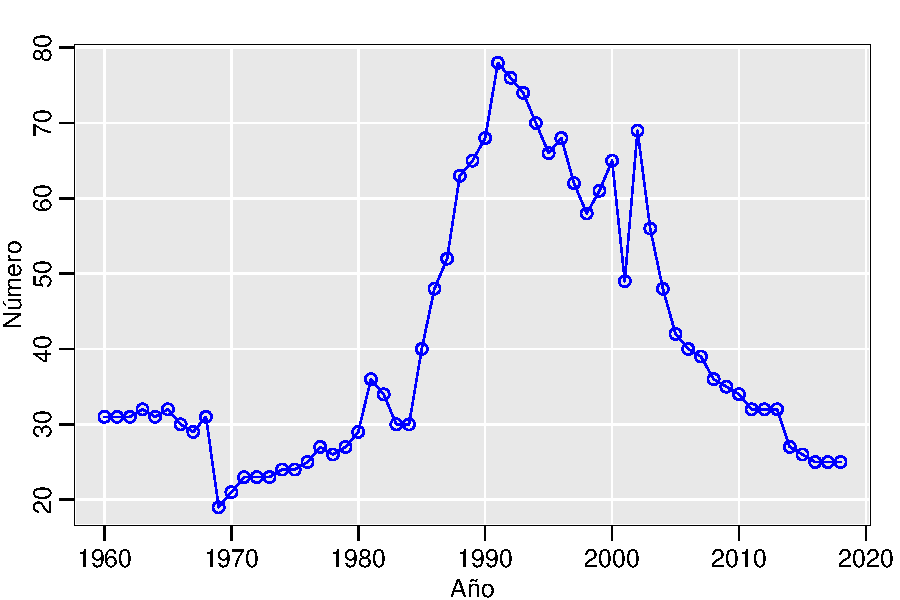
\includegraphics[width=\maxwidth]{figure/unnamed-chunk-6-1} \caption[Serie de tiempo homicidios en Colombia desde el año 1960 hasta el año 2018]{Serie de tiempo homicidios en Colombia desde el año 1960 hasta el año 2018.}\label{fig:unnamed-chunk-6}
\end{figure}


\end{knitrout}

En la figura 2, se encuentra gráficada la densidad de la serie Tasa de homicidios por 100.000 habitantes en Colombia, se deduce que utilizar modelo de regresión Poisson, sería inapropiado pues parece haber una mixtura entre dos distribuciones, ahora la pregunta que deberíamos hacernos es si estas dos distribuciones están correlacionadas, pues de no estarlo una opción para modelar esta serie sería utilizar una mixtura entre dos o más distribuciones independientes, como se muestra en Zucchini (2012, capítulo 1). Por otra parte parece haber una sobredispersión enorme pues mientras la media se sitúa en 40, la varianza es 292 es decir 7 veces la media, y recordemos que para la distribución Poisson $\mu = \sigma^2 = \lambda$. 

Un primer período de incremento acelerado que va desde comienzos de los 80, en particular desde 1983, hasta 1991. Es la fase más crítica de violencia, en particular de violencia homicida, en los anales de la ciudad. Las tasas de homicidio en la ciudad llegaron a marcar la tendencia de la curva de homicidios a nivel nacional. Investigaciones anteriores \textbf{19-22} han tratado de explicar este incremento acelerado mediante la convergencia de los problemas acumulados de debilidad institucional, ausencias estatales, ciudadanía precaria, desempleo e inequidades crecientes, con la expansión del fenómeno del narcotráfico en la ciudad \textbf{23} y su confrontación armada estatal, con la intensificación de la presencia urbana del conflicto armado interno, en especial la actuación de las milicias afines a las organizaciones guerrilleras y la emergencia y acelerado desarrollo de organizaciones paramilitares \textbf{24,25}.

\begin{knitrout}
\definecolor{shadecolor}{rgb}{0.91, 0.91, 0.91}\color{fgcolor}\begin{figure}
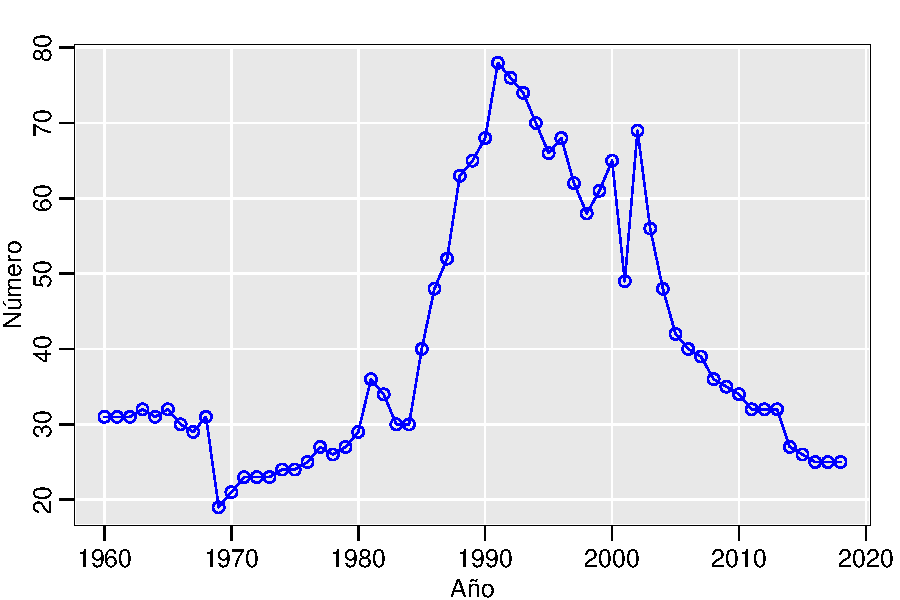
\includegraphics[width=\maxwidth]{figure/unnamed-chunk-7-1} \caption[Kernel Densidad de homicidios en Colombia (1960-2018)]{Kernel Densidad de homicidios en Colombia (1960-2018).}\label{fig:unnamed-chunk-7}
\end{figure}


\end{knitrout}

En la figura 3 se observa la función de autocorrelación muestral para la serie Tasa de homicidios hasta el rezago 30, como se evidencia existe una fuerte dependencia serial en los datos por lo que seria inapropiado utilizar un modelo de mixturas independientes (distribución Poisson), como alternativa surge la utilización de los modelos ocultos de Markov, en este caso se utilizara un PHMM.

\begin{knitrout}
\definecolor{shadecolor}{rgb}{0.91, 0.91, 0.91}\color{fgcolor}\begin{figure}
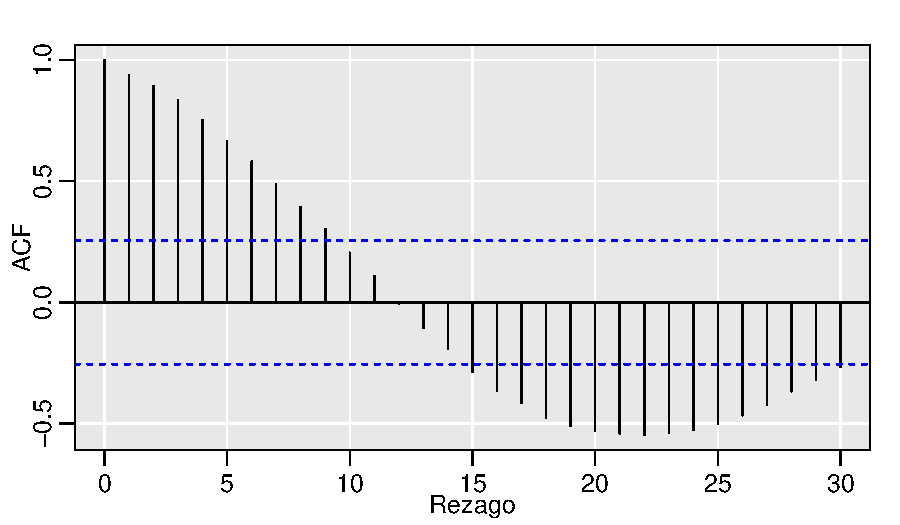
\includegraphics[width=\maxwidth]{figure/unnamed-chunk-8-1} \caption[Función de autocorrelación muetral, para la serie de homicidios]{Función de autocorrelación muetral, para la serie de homicidios.}\label{fig:unnamed-chunk-8}
\end{figure}


\end{knitrout}

\subsubsection*{Ajuste clásico PHMM}






Primero ajustamos varios modelos Poisson ocultos de Markov con 1 a 5 estados, y tres modelos con mixturas independientes con 2, 3 y 4 componentes de la distribución Poisson utilizando el paquete \textbf{flexmix} de R. Por último registramos los siguientes valores en la Tabla 3, el número de parámetros estimados, la log-verosimilitud el criterio de información de Akaike (AIC) y el criterio de información bayesiano (BIC). Con el fin de seleccionar el modelo más apropiado, el valor que minimiza el AIC es el PHMM de orden 3 con un valor de 404.02, mientras que el BIC indica que el modelo apropiado es un PHMM de orden 2, con un valor de 418.96. Tanto el BIC y AIC resuelven este problema mediante la introducción de un término de penalización para el número de parámetros en el modelo, el término de penalización es mayor en el BIC que en el AIC. El BIC generalmente penaliza parámetros libres con más fuerza que hace el criterio de información de Akaike, aunque depende del tamaño de $n$ y la magnitud relativa de $n$ y $p$. Como el tamaño de la muestra es relativamente grande $n = 59$, y la cantidad de parámetros que se estiman en un HMM es bastante utilizaremos el BIC en este caso en concreto, eligiendo por tanto el PHMM de orden 2.

% latex table generated in R 3.4.4 by xtable 1.8-4 package
% Fri Jun 21 20:26:57 2019
\begin{table}[ht]
\centering
\begin{tabular}{rlrrrr}
  \hline
 & Modelo & p & logL & AIC & BIC \\ 
  \hline
1 & PHMM - Estados 1 & 1.00 & -356.91 & 715.81 & 717.89 \\ 
  2 & PHMM - Estados 2 & 4.00 & -201.32 & 410.65 & 418.96 \\ 
  3 & PHMM - Estados 3 & 9.00 & -193.01 & 404.02 & 422.71 \\ 
  4 & PHMM - Estados 4 & 16.00 & -190.84 & 413.69 & 446.93 \\ 
  5 & PHMM - Estados 5 & 25.00 & -190.29 & 430.58 & 482.51 \\ 
  6 & mixtura indep. (2) & 3.00 & -229.38 & 464.75 & 470.98 \\ 
  7 & mixtura indep. (3) & 5.00 & -228.11 & 466.21 & 476.60 \\ 
  8 & mixtura indep. (4) & 7.00 & -228.11 & 470.21 & 484.76 \\ 
   \hline
\end{tabular}
\caption{Datos homicidios: comparación de modelos ocultos de Markov (estacionarios) por AIC y BIC.} 
\end{table}


\begin{knitrout}
\definecolor{shadecolor}{rgb}{0.91, 0.91, 0.91}\color{fgcolor}\begin{figure}[h]
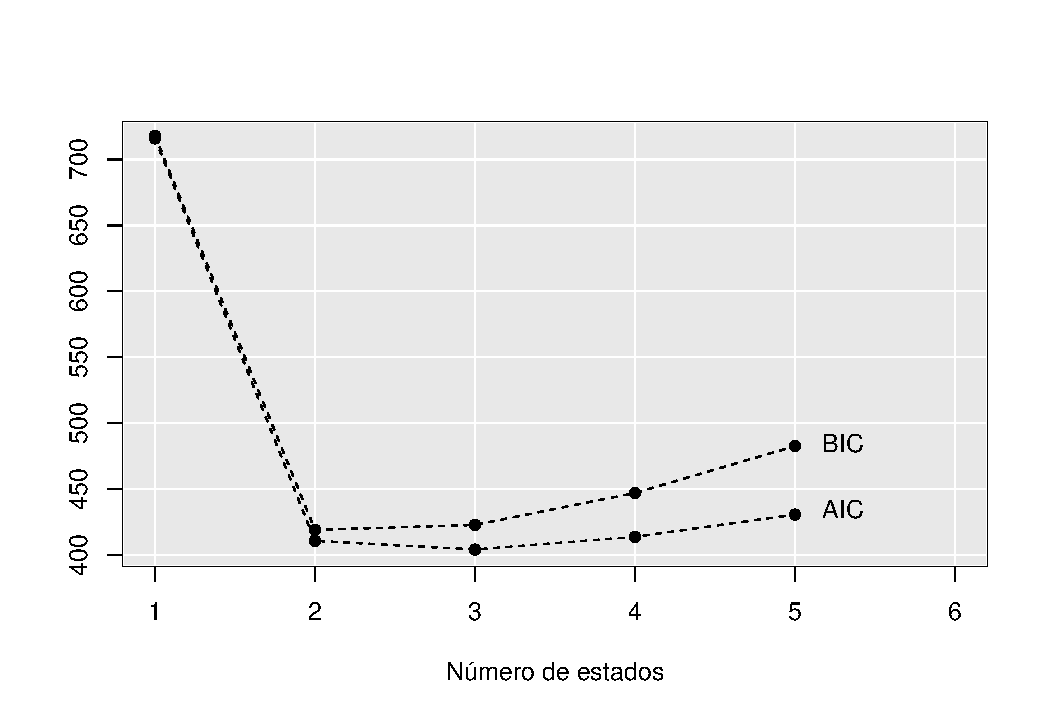
\includegraphics[width=\maxwidth]{figure/unnamed-chunk-12-1} \caption[Serie homicidios]{Serie homicidios: selección de modelos AIC y BIC.}\label{fig:unnamed-chunk-12}
\end{figure}


\end{knitrout}

Varios comentarios surgen de la Tabla 4. En primer lugar, dada la dependencia en serie manifestada en la Figura 2, no es sorprendente que los modelos de mezcla independientes no tengan un buen desempeño en relación con los HMM. En segundo lugar, aunque quizás sea obvio a priori que ni siquiera se debe intentar establecer un modelo con un máximo de 16 o 25 parámetros para 59 observaciones, y observaciones dependientes, es interesante explorar las funciones de verosimilitud en el caso de HMM con cuatro y cinco estados. La verosimilitud parece ser altamente multimodal en estos casos, y es fácil encontrar varios máximos locales utilizando diferentes valores de inicio. Una estrategia que parece tener éxito en estos casos es comenzar todas las probabilidades de transición fuera de la diagonal en valores pequeños (como 0.1 o 0.05), mientras que para los valores de las medias estado dependientes se pueden usar los valores de los deciles, calculados a partir de la variable de interés.



La estimaciones del modelo son las siguientes la media de los estados dependientes $\lambda = (29.72, 62.8)$  y los valores de la distribución estacionaria son $\pi = (0.764, 0.236)$. Ahora veamos la estimación de la matriz de transición para el modelo con 2 estados:

$$
A = \begin{pmatrix}{}
  0.980 & 0.020 \\ 
  0.064 & 0.936 \\ 
\end{pmatrix}
$$

Ahora miraremos otras metodologías alternativas a los criterios de información AIC y BIC, que determinan si el modelo tiene un buen ajuste. Entre estas es útil comparar las funciones de autocorrelación de los HMM con dos, tres, cuatro y cinco estados con la función de autocorrelación muestral (ACF). Los ACF de los modelos se pueden encontrar utilizando la función `Bayeshmmcts::pois.HMM.moments` utilizando la ecuación de Zucchini, pág. 55. En forma tabular los ACF se muestran en la tabla 5:

% latex table generated in R 3.4.4 by xtable 1.8-4 package
% Fri Jun 21 20:26:57 2019
\begin{table}[ht]
\centering
\begin{tabular}{rrrrrrrrrrrrr}
  \hline
 & 1 & 2 & 3 & 4 & 5 & 6 & 7 & 8 & 9 & 10 & 11 & 12 \\ 
  \hline
observaciones & 0.94 & 0.89 & 0.83 & 0.75 & 0.67 & 0.58 & 0.49 & 0.39 & 0.30 & 0.20 & 0.11 & -0.01 \\ 
  PHMM 2 Estados & 0.77 & 0.71 & 0.65 & 0.59 & 0.54 & 0.50 & 0.46 & 0.42 & 0.38 & 0.35 & 0.32 & 0.29 \\ 
  PHMM 3 Estados & 0.79 & 0.75 & 0.71 & 0.68 & 0.64 & 0.61 & 0.58 & 0.55 & 0.52 & 0.50 & 0.47 & 0.45 \\ 
  PHMM 4 Estados & 0.80 & 0.76 & 0.72 & 0.69 & 0.65 & 0.62 & 0.58 & 0.55 & 0.52 & 0.49 & 0.47 & 0.44 \\ 
   \hline
\end{tabular}
\caption{Datos homicidios: ACF y ACF de los cuatro modelos hasta el rezago 12.} 
\end{table}


\begin{knitrout}
\definecolor{shadecolor}{rgb}{0.91, 0.91, 0.91}\color{fgcolor}\begin{figure}[h]
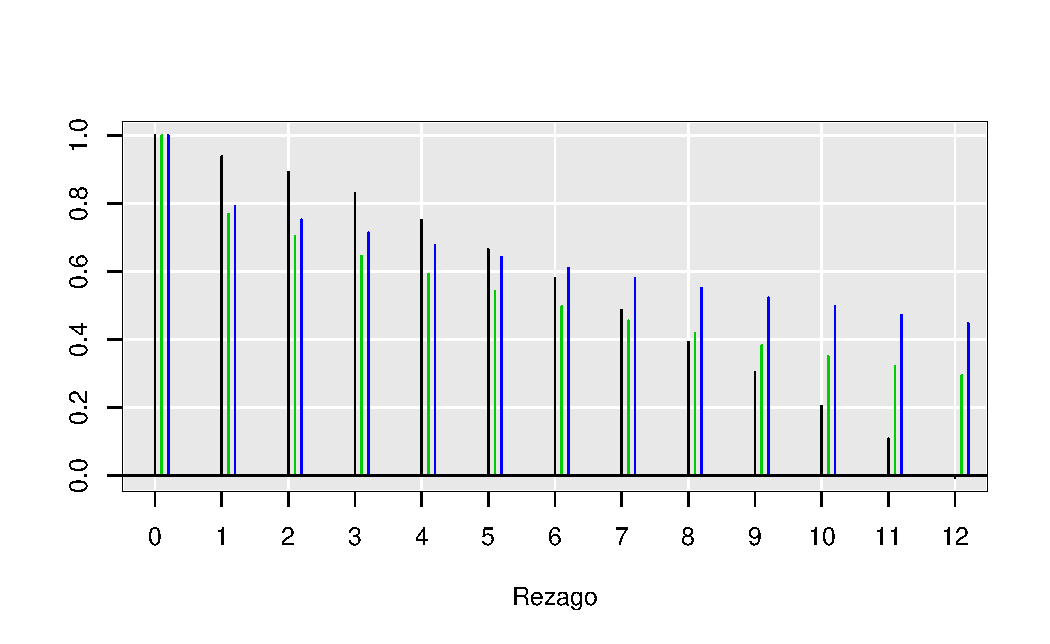
\includegraphics[width=\maxwidth]{figure/unnamed-chunk-15-1} \caption[Datos homicidios]{Datos homicidios: ACF y ACF de los PHMM con dos y tres estados.}\label{fig:unnamed-chunk-15}
\end{figure}


\end{knitrout}

En la Figura 6, de izquierda a derecha se muestran el ACF de las observaciones, la barra de color verde pertenece al modelo de dos estados y la azul al modelo de tres estados. Nos interesa ver como está yuxtapuesto los ACF de ambos modelos con respecto al ACF de las observaciones. Está claro que los ACF del modelo con tres estados corresponden bien con el ACF de las observaciones hasta aproximadamente el rezago 6, mientras que el modelo 2 estados coincide hasta el rezago 9. Sin embargo, se pueden aplicar diagnósticos más sistemáticos, como se mostrará a continuación.

\subsubsection*{Verificación de supuestos del PHMM}

En este caso hemos elegido el BIC como criterio para la selección del mejor modelo como mostramos anteriormente, sin embargo sigue existiendo el problema de decidir si el modelo es realmente adecuado; por lo tanto se necesitan herramientas para evaluar la bondad general del ajuste del modelo e identificar valores atípicos en relación con el modelo. En el contexto más simple como por ejemplo los modelos de regresión (teoría normal), el papel que juegan los residuales como herramienta para la verificación del supuesto del modelo está muy bien establecido, entre estos supuestos están la normalidad de los residuales, la homocedasticidad y la independencia de estos. Los pseudo-residuos (también conocidos como residuos quantílicos) que se ilustraron en la sección tres tienen la intención de cumplir esta función de manera mucho más general, y que son útiles en el contexto de los HMM. 

\begin{knitrout}
\definecolor{shadecolor}{rgb}{0.91, 0.91, 0.91}\color{fgcolor}\begin{figure}[h]
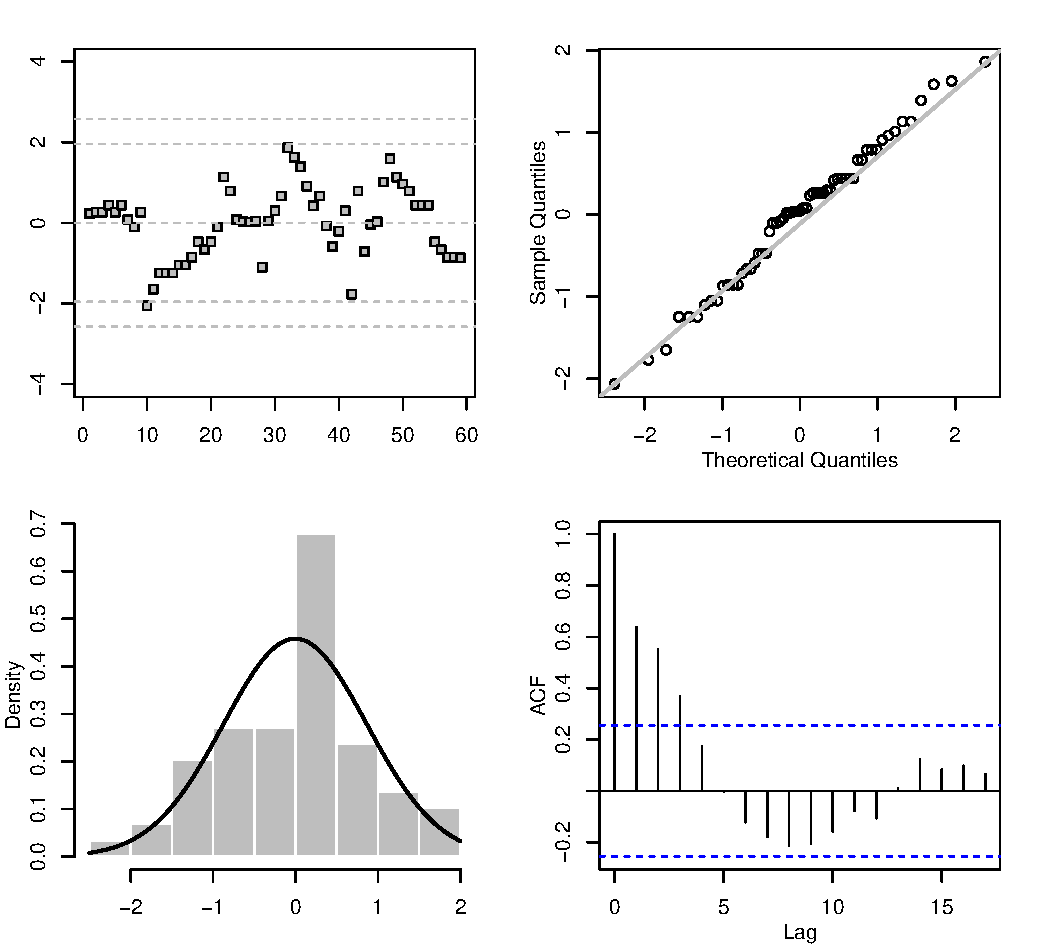
\includegraphics[width=\maxwidth]{figure/unnamed-chunk-16-1} \caption[Grafico pseudo-residuales ordinarios para el PHMM de 2 estados]{Grafico pseudo-residuales ordinarios para el PHMM de 2 estados.}\label{fig:unnamed-chunk-16}
\end{figure}


\end{knitrout}

En el gráfico 6, se muestra los pseudo residuales ordinarios del PHMM con 2 estados. La fila superior izquierda muestra el diagramas de índice de los pseudo-residuos normales, con líneas horizontales en 0, $\pm 1.96$ y $\pm 2.58$. En la parte superior derecha se muestra los gráficos de cuantiles-cuantiles de los pseudo-residuos normales, con los cuantiles teóricos en el eje $x$. La última fila muestra en la parte izquierda el histograma de los pseudo residuales normales, y en la parte derecha la función de autocorrelación muestral de los pseudo-residuos normales. Efectivamente los pseudo-residuales parecen distribuirse normalmente, sin embargo realizamos la prueba de Shapiro-Wilks para verificar este supuesto, donde el p-valor es 0.7529, por lo tanto no podemos rechazar la hipótesis nula $H_0$, y concluimos que hay suficiente evidencia estadística para decir que los pseudo-residuos se distribuyen normalmente con un nivel de confianza del 95\%. Además todos los puntos están dentro de las bandas de confianza, sin embargo el histograma no parece acomodarse en todos sus puntos a la curva de la distribución normal, y el mayor problema es que los pseudo-residuales parecen estar correlacionados, hasta el rezago 3.

\subsubsection*{Algoritmo Viterbi}

El algoritmo Viterbi, permite realizar la decodificación global de los estados clasificando a cada una de las observaciones en su correspondiente estado, dando como resultado la anterior tabla, para un total de 40 observaciones en el estado 1 y 19 en el estado 2. En la grafica 5 se visualiza el algoritmo viterbi.

% latex table generated in R 3.4.4 by xtable 1.8-4 package
% Fri Jun 21 20:26:57 2019
\begin{table}[ht]
\centering
\begin{tabular}{rrrrrrrrrrrrrrrrrrrr}
  \hline
  \hline
1 & 1 & 1 & 1 & 1 & 1 & 1 & 1 & 1 & 1 & 1 & 1 & 1 & 1 & 1 & 1 & 1 & 1 & 1 & 1 \\ 
  1 & 1 & 1 & 1 & 1 & 1 & 2 & 2 & 2 & 2 & 2 & 2 & 2 & 2 & 2 & 2 & 2 & 2 & 2 & 2 \\ 
  2 & 2 & 2 & 2 & 2 & 1 & 1 & 1 & 1 & 1 & 1 & 1 & 1 & 1 & 1 & 1 & 1 & 1 & 1 &  \\ 
   \hline
\end{tabular}
\caption{Resultados de la decodificación global con el algoritmo Viterbi.} 
\end{table}


\begin{knitrout}
\definecolor{shadecolor}{rgb}{0.91, 0.91, 0.91}\color{fgcolor}\begin{figure}
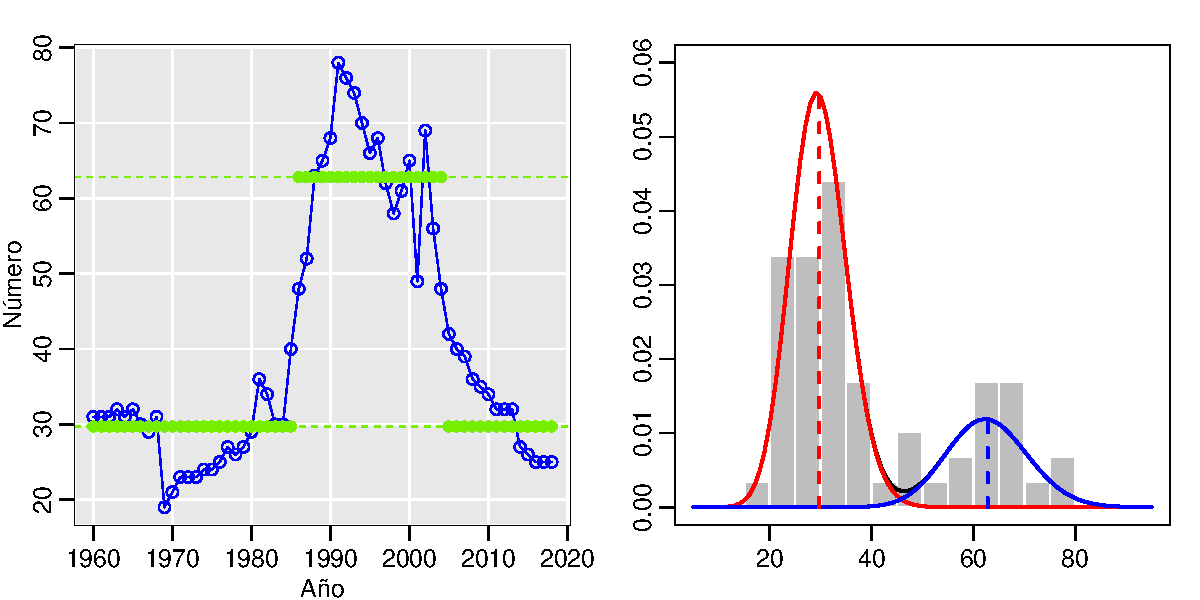
\includegraphics[width=\maxwidth]{figure/unnamed-chunk-18-1} \caption[Algoritmo Viterbi aplicado a un PHMM de dos estados]{Algoritmo Viterbi aplicado a un PHMM de dos estados.}\label{fig:unnamed-chunk-18}
\end{figure}


\end{knitrout}

Ahora realizaremos la predicción de los estados más probables para los proximos 12 años, tambien podemos pronosticar la distribución para estos mismos años. Como se observa en la figura () a medida que el horizonte de pronóstico $h$ aumenta, la distribución de pronóstico converge a la distribución marginal del HMM estacionario.

% latex table generated in R 3.4.4 by xtable 1.8-4 package
% Fri Jun 21 20:26:57 2019
\begin{table}[ht]
\centering
\begin{tabular}{rrrr}
  \hline
 & Estado 1 & Estado 2 & Estado \\ 
  \hline
2019 & 0.9802 & 0.0198 &     1 \\ 
  2020 & 0.9621 & 0.0379 &     1 \\ 
  2021 & 0.9456 & 0.0544 &     1 \\ 
  2022 & 0.9304 & 0.0696 &     1 \\ 
  2023 & 0.9164 & 0.0836 &     1 \\ 
  2024 & 0.9037 & 0.0963 &     1 \\ 
  2025 & 0.8920 & 0.1080 &     1 \\ 
  2026 & 0.8813 & 0.1187 &     1 \\ 
  2027 & 0.8714 & 0.1286 &     1 \\ 
  2028 & 0.8624 & 0.1376 &     1 \\ 
  2029 & 0.8542 & 0.1458 &     1 \\ 
  2030 & 0.8467 & 0.1533 &     1 \\ 
   \hline
\end{tabular}
\caption{Predicción para las probabilidades de los estados hasta un rezago h = 12.} 
\end{table}


\begin{knitrout}
\definecolor{shadecolor}{rgb}{0.91, 0.91, 0.91}\color{fgcolor}\begin{figure}
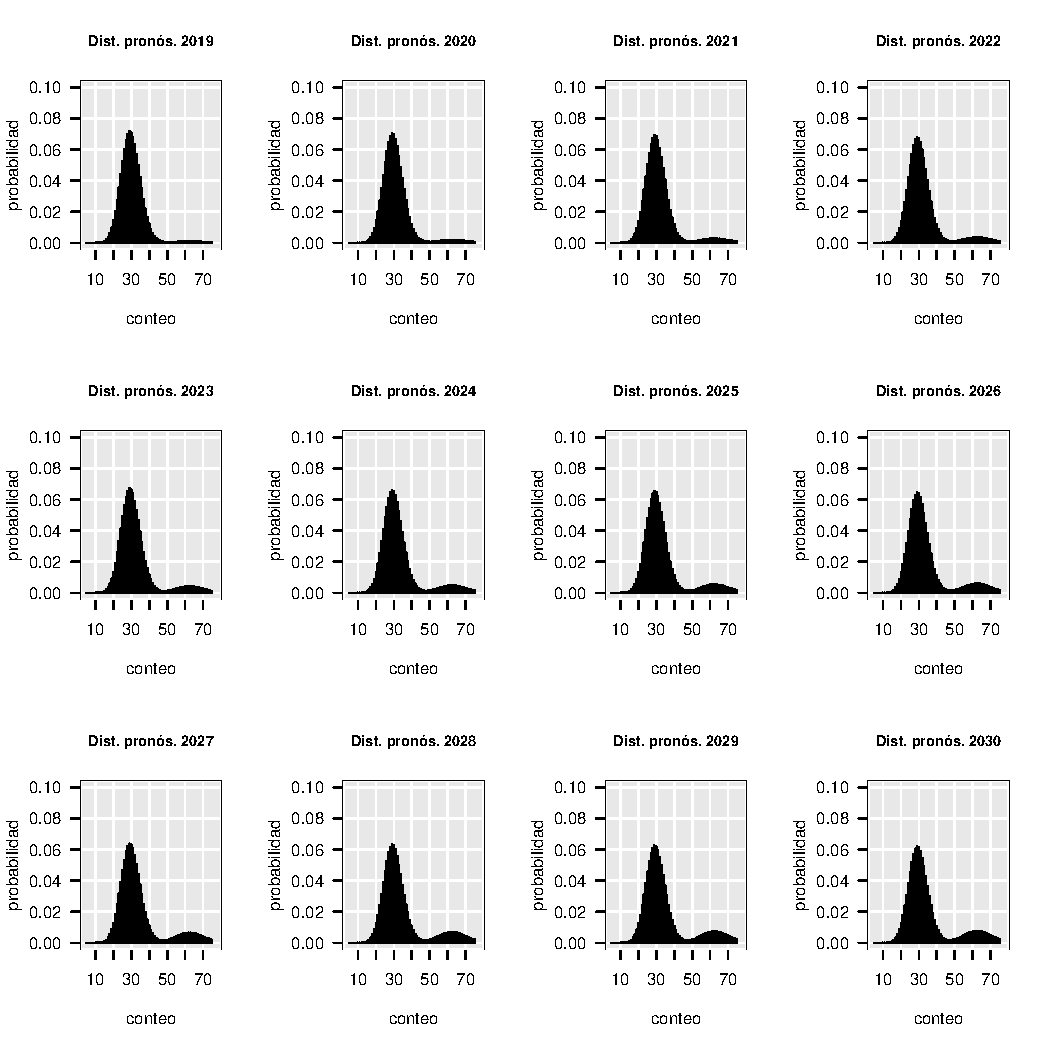
\includegraphics[width=\maxwidth]{figure/unnamed-chunk-20-1} \caption[Pronostico de la distribución para los años 2019 a 2030]{Pronostico de la distribución para los años 2019 a 2030.}\label{fig:unnamed-chunk-20}
\end{figure}


\end{knitrout}


\begin{knitrout}
\definecolor{shadecolor}{rgb}{0.91, 0.91, 0.91}\color{fgcolor}\begin{figure}[t]
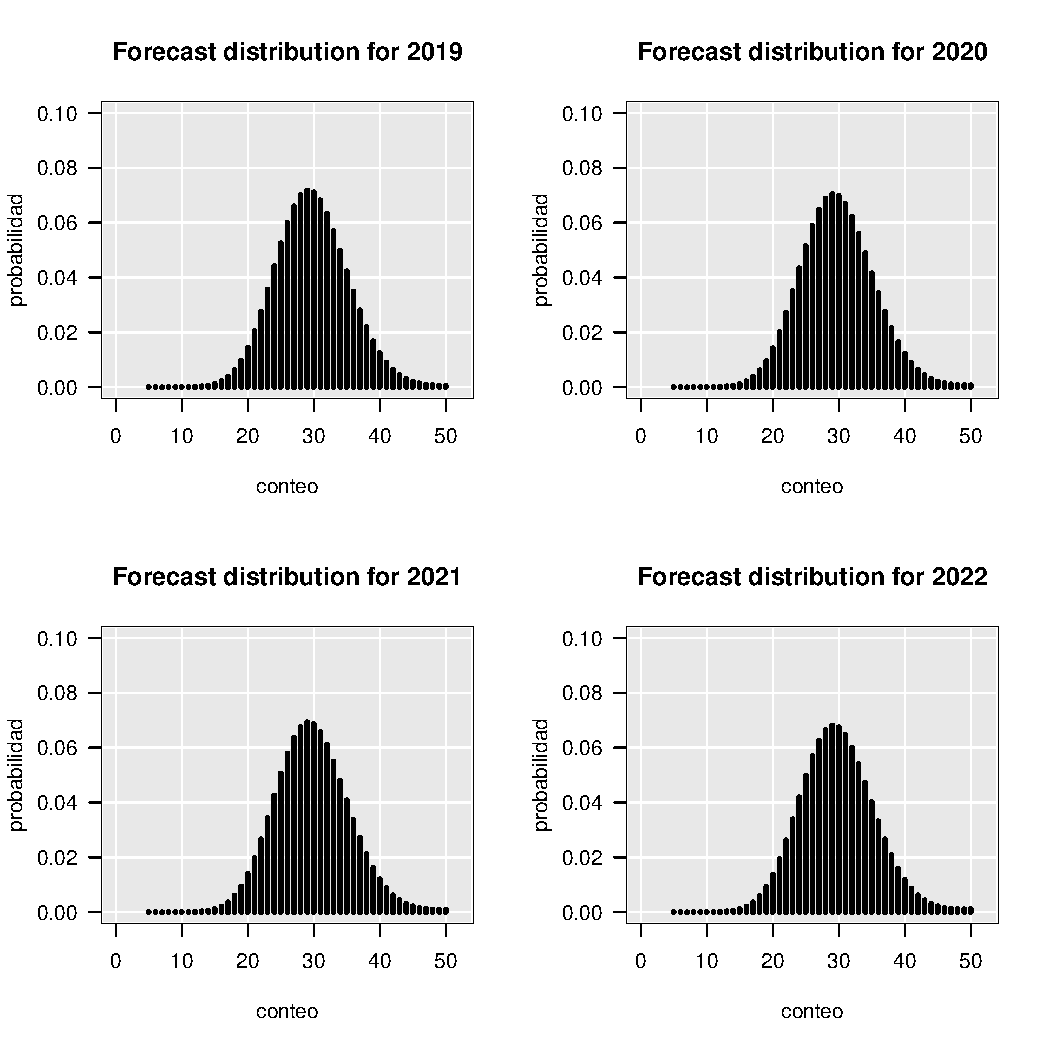
\includegraphics[width=\maxwidth]{figure/unnamed-chunk-21-1} \caption[La distribución prónosticada para el año 2098]{La distribución prónosticada para el año 2098}\label{fig:unnamed-chunk-21}
\end{figure}


\end{knitrout}

%http://www.scielo.br/pdf/csc/v17n12/06.pdf

\clearpage

\subsubsection*{Estimación Bayesiana del PHMM}





Primero se ajustaron cuatro modelos, con la función `Bayeshmmcts::bayes.PHMM`, para 2, 3, 4 y 5 estados, después, se estimo la $\log$ - verosimilitud marginal, utilizando muestreo por puente como alternativa a las propuesta hecha por Newton y Raftery (1994) que sugiere utilizar la verosimilitud integrada, para hallar el estimador de la media armónica de los valores de la verosimilitud de una muestra obtenida desde la distribución posterior. Pero como se vio en la sección (4), aunque el estimador es consitente tiene un gran problema varianza infinita. Mientras que el estimador de muestreo por puente, no presenta ese problema además de su facil implementación, pues esta metodología se puede ejecutar con la función ` bridge sampler` del paquete bridgesampling, del autor Gronau. Inclusive calcular el error para la verosimilitud marginal, que en el caso del modelo con dos estados es de $0.478 \%$, mientras que para el modelo de 3 estados el error es de $3.11 \%$ aunque es más alto, sigue siendo relativamente bajo. Después utilizamos el factor de bayes para contrastar los modelos con m-estados de a parejas, y seleccionar el más adecuado, la siguiente tabla ilustra el contraste de hipótesis:

% latex table generated in R 3.4.4 by xtable 1.8-4 package
% Fri Jun 21 20:26:57 2019
\begin{table}[ht]
\centering
\begin{tabular}{rrrrr}
  \hline
 & mod 2 Estados & mod 3 Estados & mod 4 Estados & mod 5 Estados \\ 
  \hline
mod 2 Estados &  & 3.36 & 3047.46 & 390147608.00 \\ 
  mod 3 Estados &  &  & 980.61 & 125542040.00 \\ 
  mod 4 Estados &  &  &  & 128023.00 \\ 
   \hline
\end{tabular}
\caption{Comparación resultados Factor de Bayes.} 
\end{table}




Por lo tanto se ajusta un PHMM de orden 2 lo cual coincide con la teoría clásica. Se corrieron 5.000 iteraciones con 3 cadenas y las primeras 2.500 iteraciones de calentamiento adelgazando la cadena cada 3 iteraciones; con tasa de aceptación para la función objetivo en el metropolis de 0.99. A continuación mostramos las estimaciones bayesianas de la matriz de transición, y la media de los estados dependiesntes:

% latex table generated in R 3.4.4 by xtable 1.8-4 package
% Fri Jun 21 20:26:57 2019
\begin{table}[ht]
\centering
\begin{tabular}{rrrrrrrrrrr}
  \hline
 & mean & se\_mean & sd & 2.5\% & 25\% & 50\% & 75\% & 97.5\% & n\_eff & Rhat \\ 
  \hline
Gamma[1,1] & 0.95 & 0.00 & 0.03 & 0.87 & 0.94 & 0.96 & 0.98 & 0.99 & 2489.68 & 1.00 \\ 
  Gamma[1,2] & 0.05 & 0.00 & 0.03 & 0.01 & 0.02 & 0.04 & 0.06 & 0.13 & 2489.68 & 1.00 \\ 
  Gamma[2,1] & 0.10 & 0.00 & 0.06 & 0.01 & 0.05 & 0.08 & 0.13 & 0.25 & 2241.08 & 1.00 \\ 
  Gamma[2,2] & 0.90 & 0.00 & 0.06 & 0.75 & 0.87 & 0.92 & 0.95 & 0.99 & 2241.08 & 1.00 \\ 
  lambda[1] & 29.71 & 0.02 & 0.88 & 27.97 & 29.11 & 29.73 & 30.31 & 31.41 & 2270.72 & 1.00 \\ 
  lambda[2] & 62.75 & 0.04 & 1.94 & 58.95 & 61.43 & 62.74 & 64.02 & 66.44 & 2647.06 & 1.00 \\ 
  lp\_\_ & -210.61 & 0.03 & 1.48 & -214.32 & -211.32 & -210.28 & -209.52 & -208.75 & 2051.34 & 1.00 \\ 
   \hline
\end{tabular}
\end{table}


% latex table generated in R 3.4.4 by xtable 1.8-4 package
% Fri Jun 21 20:26:58 2019
\begin{table}[ht]
\centering
\begin{tabular}{rrrrrrrrrrrrrrrrrrrr}
  \hline
  \hline
1 & 1 & 1 & 1 & 1 & 1 & 1 & 1 & 1 & 1 & 1 & 1 & 1 & 1 & 1 & 1 & 1 & 1 & 1 & 1 \\ 
  1 & 1 & 1 & 1 & 1 & 1 & 2 & 2 & 2 & 2 & 2 & 2 & 2 & 2 & 2 & 2 & 2 & 2 & 2 & 2 \\ 
  2 & 2 & 2 & 2 & 2 & 1 & 1 & 1 & 1 & 1 & 1 & 1 & 1 & 1 & 1 & 1 & 1 & 1 & 1 &  \\ 
   \hline
\end{tabular}
\caption{Resultados de la decodificación global bayesiana con el algoritmo Viterbi.} 
\end{table}


\begin{knitrout}
\definecolor{shadecolor}{rgb}{0.91, 0.91, 0.91}\color{fgcolor}\begin{figure}
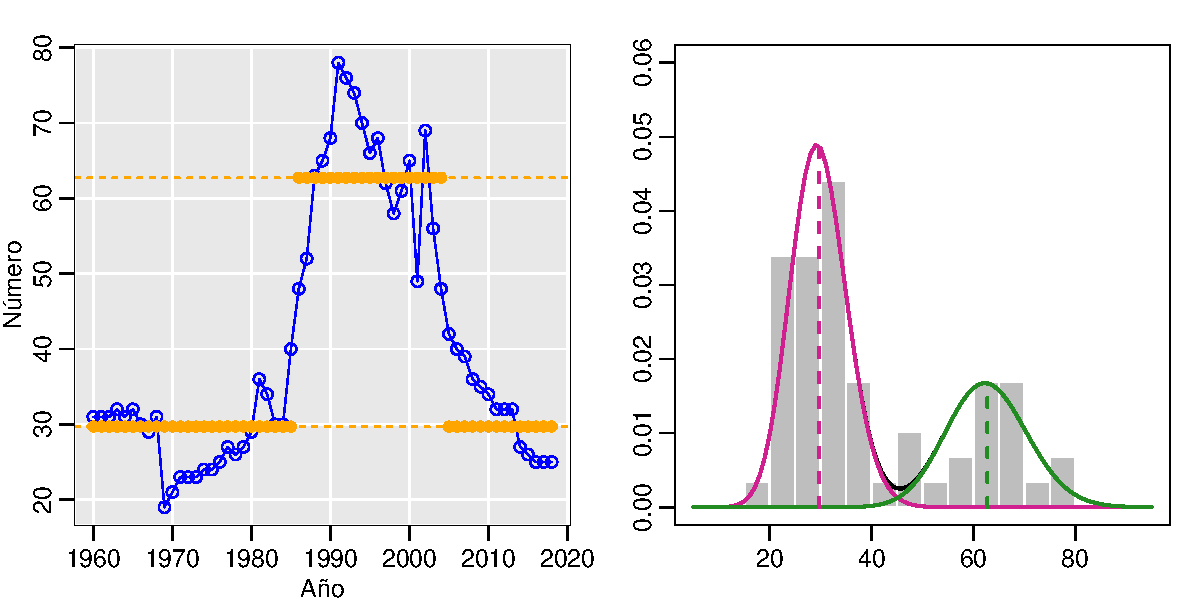
\includegraphics[width=\maxwidth]{figure/unnamed-chunk-28-1} \caption[Algoritmo Viterbi aplicado a un PHMM de dos estados]{Algoritmo Viterbi aplicado a un PHMM de dos estados.}\label{fig:unnamed-chunk-28}
\end{figure}


\end{knitrout}

% latex table generated in R 3.4.4 by xtable 1.8-4 package
% Fri Jun 21 20:26:58 2019
\begin{table}[ht]
\centering
\begin{tabular}{rrrr}
  \hline
 & Estado 1 & Estado 2 & Estado \\ 
  \hline
2019 & 0.9517 & 0.0483 &     1 \\ 
  2020 & 0.9104 & 0.0896 &     1 \\ 
  2021 & 0.8751 & 0.1249 &     1 \\ 
  2022 & 0.8449 & 0.1551 &     1 \\ 
  2023 & 0.8191 & 0.1809 &     1 \\ 
  2024 & 0.7971 & 0.2029 &     1 \\ 
  2025 & 0.7783 & 0.2217 &     1 \\ 
  2026 & 0.7622 & 0.2378 &     1 \\ 
  2027 & 0.7484 & 0.2516 &     1 \\ 
  2028 & 0.7366 & 0.2634 &     1 \\ 
  2029 & 0.7266 & 0.2734 &     1 \\ 
  2030 & 0.7180 & 0.2820 &     1 \\ 
   \hline
\end{tabular}
\caption{Predicción bayesiana para las probabilidades de los estados hasta un rezago h = 12.} 
\end{table}


\subsubsection*{Diagnosticos de la cadena}

En esta sección se verificara el diagnostico de convergencia de las cadenas utilizadas en la extracción de las muestras. Para los métodos MCMC ajustados con \textbf{Stan}, ya sean Hamiltonian Monte (HMC) o No-U-Turn-Sampler (NUTS), el paquete \emph{bayesplot} y \emph{coda}, cuenta con una serie de herrmientas gráficas y purebas diagnosticas para después del ajuste de modelos bayesianos. En la figura No se muestra los histogramas univariados y diagramas de dispersión bivariados para los parámetros de la matriz de transición de probabilidad y para el vector de medias de los estados dependientes, especialmente útil para identificar la colinealidad entre variables (que se manifiesta como gráficos bivariados estrechos), así como la presencia de no-identificabilidad multiplicativa (formas tipo plátano).

En sentido estricto, la no identificabilidad significa que dos valores de los parámetros dan como resultado la misma distribución de probabilidad de los datos observados. Algunas veces también se usa para cubrir situaciones en las que no hay un máximo local único de la densidad posterior, ya sea porque hay múltiples máximos separados o porque hay una meseta donde un conjunto de puntos tiene la misma densidad posterior (estos pueden o pueden No ser identificable en sentido estricto).

En este caso parece no haber problemas con la identificabilidad, es decir que no existen problemas que señalan divergencias, lo único que se observa es colinealidad entre los parámetros de las filas de la matriz de transición, sin embargo recordemos por definición que la suma de las filas de la tpm suman 1, por lo tanto están de por si correlacionadas. Por lo tanto como el modelo es identificable, no estamos asegurando que las inferencias no están sesgadas.

\begin{knitrout}
\definecolor{shadecolor}{rgb}{0.91, 0.91, 0.91}\color{fgcolor}\begin{figure}
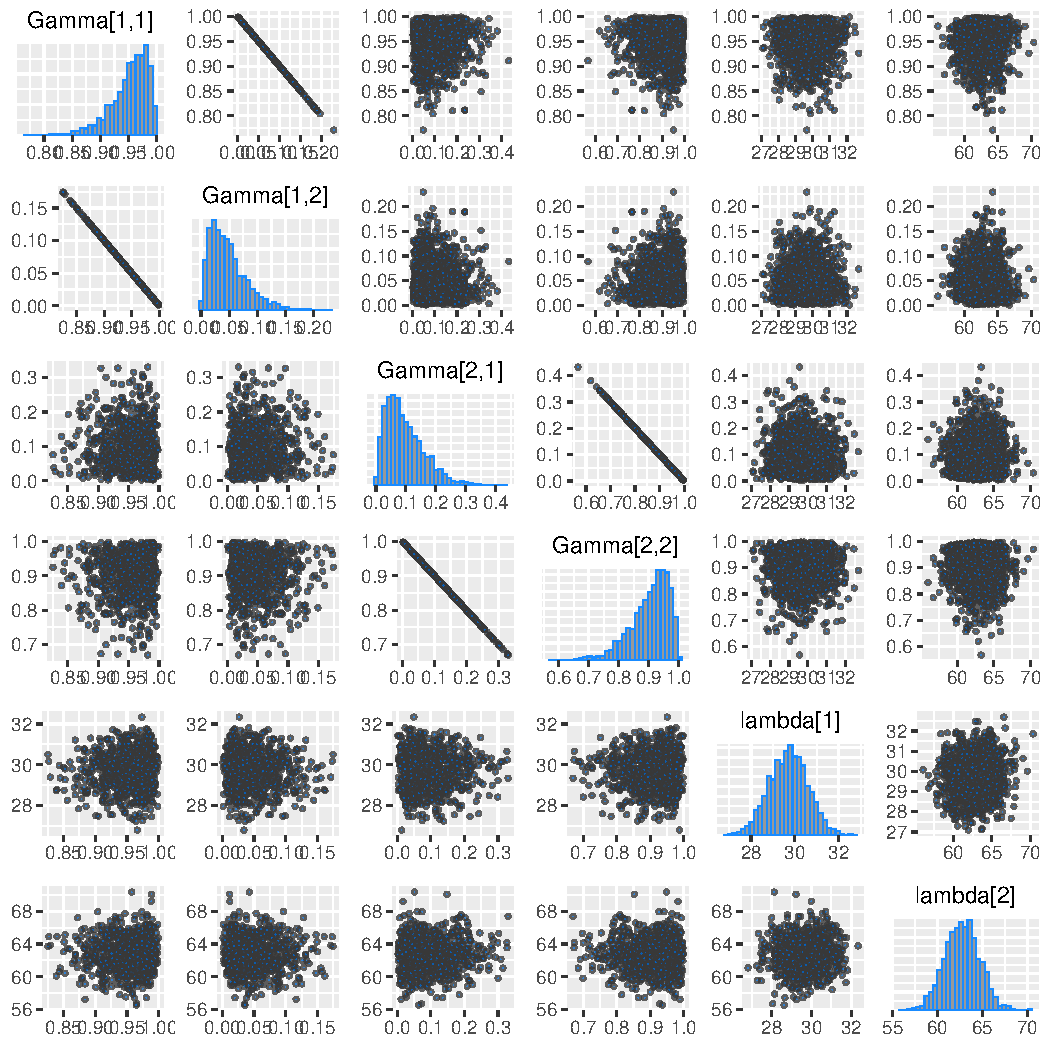
\includegraphics[width=\maxwidth]{figure/unnamed-chunk-30-1} \caption[Gráfico de dispersión para las muestras MCMC]{Gráfico de dispersión para las muestras MCMC.}\label{fig:unnamed-chunk-30}
\end{figure}


\end{knitrout}

El gráfico de traza, muestra por cada una de las iteraciones los valores muestreados correspondiente a una o más cadenas de Markov, separado por parámetro. Las cadenas proporcionan una forma visual para inspeccionar el comportamiento de muestreo y evaluar la mezcla a través de las cadenas y la convergencia, como vemos se comportana bastante bien, pues hay un mínimo de muestras divergentes.

\begin{knitrout}
\definecolor{shadecolor}{rgb}{0.91, 0.91, 0.91}\color{fgcolor}\begin{figure}
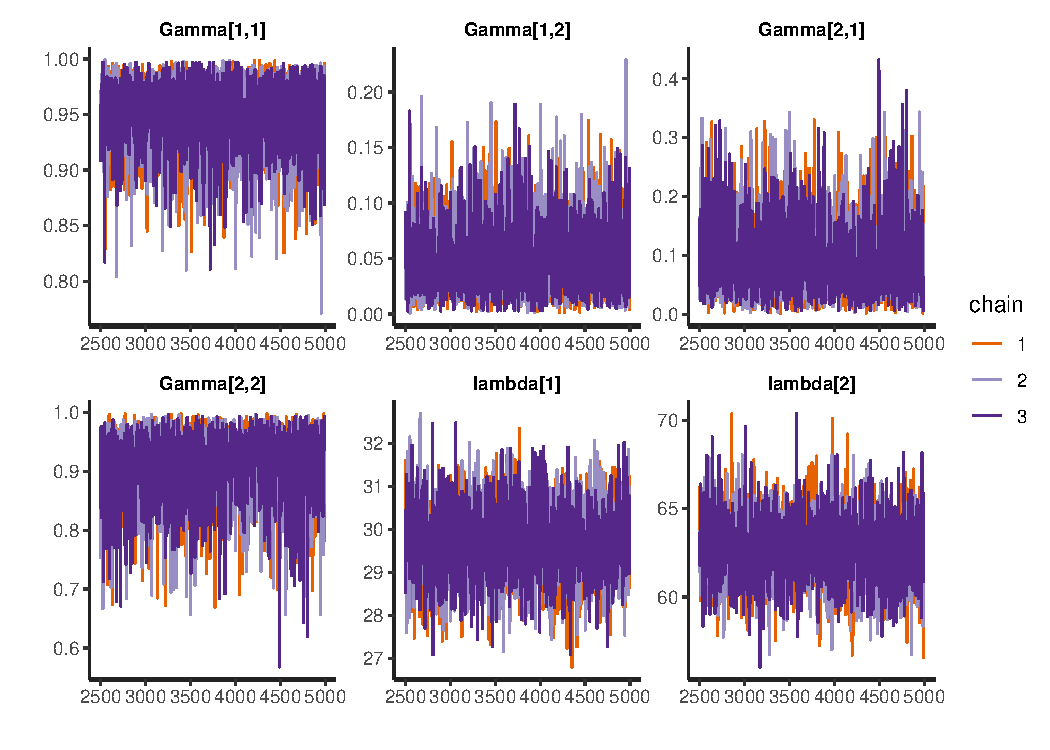
\includegraphics[width=\maxwidth]{figure/unnamed-chunk-31-1} \caption[Gráfico de trazas de las cadenas, para cada iteración y por cadena]{Gráfico de trazas de las cadenas, para cada iteración y por cadena.}\label{fig:unnamed-chunk-31}
\end{figure}


\end{knitrout}
                              
Los intervalos de credibilidad, para los parámetros calculados a partir de las muestras posteriores con todas las cadenas fusionadas. Índican valores consistentes en las estimaciones de los parámetros.

\begin{knitrout}
\definecolor{shadecolor}{rgb}{0.91, 0.91, 0.91}\color{fgcolor}\begin{figure}
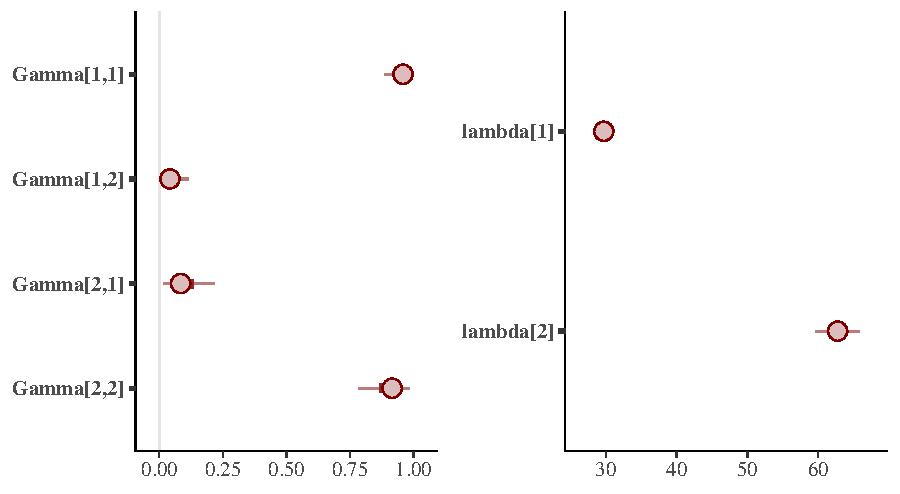
\includegraphics[width=\maxwidth]{figure/unnamed-chunk-32-1} \caption[Intervalos de crédibilidad]{Intervalos de crédibilidad.}\label{fig:unnamed-chunk-32}
\end{figure}


\end{knitrout}

La prueba de convergencia utiliza la estadística de Cramer-von-Mises para probar la hipótesis nula de que los valores muestreados provienen de una distribución estacionaria. La prueba se aplica sucesivamente, primero a toda la cadena, luego, después de descartar el primer $10 \%$, $20 \%$, ... de la cadena hasta que se acepte la hipótesis nula, o se haya descartado el $50 \%$ de la cadena. El último resultado constituye un \emph{fallo} de la prueba de estacionariedad e indica que se necesita una ejecución MCMC más larga. Si se pasa la prueba de estacionariedad, se informa el número de iteraciones a mantener y el número a descartar.

La prueba de ancho medio para la media calcula un intervalo de confianza del $95 \%$ para la media, utilizando la parte de la cadena que pasó la prueba de estacionariedad. La mitad del ancho de este intervalo se compara con la estimación de la media. Si la relación entre la mitad del ancho y la media es menor que \emph{eps}, se pasa la prueba de la mitad del ancho. De lo contrario, la longitud de la muestra no se considera lo suficientemente larga como para estimar la media con suficiente precisión.

% latex table generated in R 3.4.4 by xtable 1.8-4 package
% Fri Jun 21 20:27:09 2019
\begin{table}[ht]
\centering
\begin{tabular}{rlr}
  \hline
 & P. Estacionariedad & Valor p \\ 
  \hline
$\Gamma_{11}$ & páso & 0.40 \\ 
  $\Gamma_{21}$ & páso & 0.98 \\ 
  $\Gamma_{12}$ & páso & 0.40 \\ 
  $\Gamma_{22}$ & páso & 0.98 \\ 
  $\lambda_1$ & páso & 0.57 \\ 
  $\lambda_2$ & páso & 0.86 \\ 
  lp & páso & 0.44 \\ 
   \hline
\end{tabular}
\caption{Prueba de estacionariedad, usando el estadístico de Cramer-von-Mises para la convergencia de la cadena.} 
\end{table}
% latex table generated in R 3.4.4 by xtable 1.8-4 package
% Fri Jun 21 20:27:09 2019
\begin{table}[ht]
\centering
\begin{tabular}{rlrr}
  \hline
 & P..Medio.ancho & Media & Valor.p \\ 
  \hline
$\Gamma_{11}$ & páso & 0.95 & 0.00 \\ 
  $\Gamma_{21}$ & páso & 0.10 & 0.00 \\ 
  $\Gamma_{12}$ & páso & 0.05 & 0.00 \\ 
  $\Gamma_{22}$ & páso & 0.90 & 0.00 \\ 
  $\lambda_1$ & páso & 29.70 & 0.03 \\ 
  $\lambda_2$ & páso & 62.74 & 0.08 \\ 
  lp & páso & -210.53 & 0.06 \\ 
   \hline
\end{tabular}
\caption{Test de medio ancho para la media calculando el intervalo de confianza al 95 %.} 
\end{table}



\subsubsection{Comparación PHMM clásico vs Bayesiano}

\begin{knitrout}
\definecolor{shadecolor}{rgb}{0.91, 0.91, 0.91}\color{fgcolor}\begin{kframe}
\begin{verbatim}
## [1] 9998
\end{verbatim}
\end{kframe}
\end{knitrout}

\subsection{Modelo Poisson Cero inflado - Oculto de Markov}



En esta sección utilizaremos, los datos de incendios forestales en Colombia, desde enero del 2001 hasta diciembre del 2016.  La variable de interés es el número de grandes incendios forestales (GIF), que son aquellos incendios que superan las 500 hectáreas forestales afectadas. La periodicidad de los datos es mensual con un total 180 observaciones, en la Tabla 11 se muestran los primeros 12 registros, mientras que la Tabla 12 indica la frecuencia. Allí observamos que hay una alta proporción de ceros en los datos, pues de las 180 observaciones 124 son cero, es decir el $68.9 \%$ de los registros. Por otra parte el número máximo de GIF ocurridos en Colombia fue 23 en febrero del 2017, seguido de 20 en enero del 2010 y en tercer puesto 18 incendios para marzo del 2016, además el promedio de GIF se ubico en $1.3 \pm 3.5$ incendio por mes.

% latex table generated in R 3.4.4 by xtable 1.8-4 package
% Fri Jun 21 20:27:10 2019
\begin{table}[ht]
\centering
\begin{tabular}{rlr}
  \hline
 & Fecha & GIF \\ 
  \hline
1 & 2002-01 &   0 \\ 
  2 & 2002-02 &   1 \\ 
  3 & 2002-03 &   4 \\ 
  4 & 2002-04 &   0 \\ 
  5 & 2002-05 &   0 \\ 
  6 & 2002-06 &   0 \\ 
  7 & 2002-07 &   0 \\ 
  8 & 2002-08 &   0 \\ 
  9 & 2002-09 &   0 \\ 
  10 & 2002-10 &   0 \\ 
  11 & 2002-11 &   0 \\ 
  12 & 2002-12 &   0 \\ 
   \hline
\end{tabular}
\caption{Grandes Incendios forestales, en Colombia desde enero del 2002 a diceiembre del 2016.} 
\end{table}


% latex table generated in R 3.4.4 by xtable 1.8-4 package
% Fri Jun 21 20:27:10 2019
\begin{table}[ht]
\centering
\begin{tabular}{rrr}
  \hline
 & Conteo & Proporción \\ 
  \hline
0 & 124.00 & 0.69 \\ 
  1 & 19.00 & 0.11 \\ 
  2 & 9.00 & 0.05 \\ 
  3 & 8.00 & 0.04 \\ 
  4 & 6.00 & 0.03 \\ 
  5 & 1.00 & 0.01 \\ 
  6 & 5.00 & 0.03 \\ 
  8 & 1.00 & 0.01 \\ 
  10 & 2.00 & 0.01 \\ 
  11 & 1.00 & 0.01 \\ 
  16 & 1.00 & 0.01 \\ 
  18 & 1.00 & 0.01 \\ 
  20 & 1.00 & 0.01 \\ 
  23 & 1.00 & 0.01 \\ 
   \hline
\end{tabular}
\caption{Tabla de frecuencia para la base GIF Colombia (2002-2016).} 
\end{table}


Se quiere determinar si existe correlación entre los GIF de cada mes, 

\begin{knitrout}
\definecolor{shadecolor}{rgb}{0.91, 0.91, 0.91}\color{fgcolor}\begin{figure}
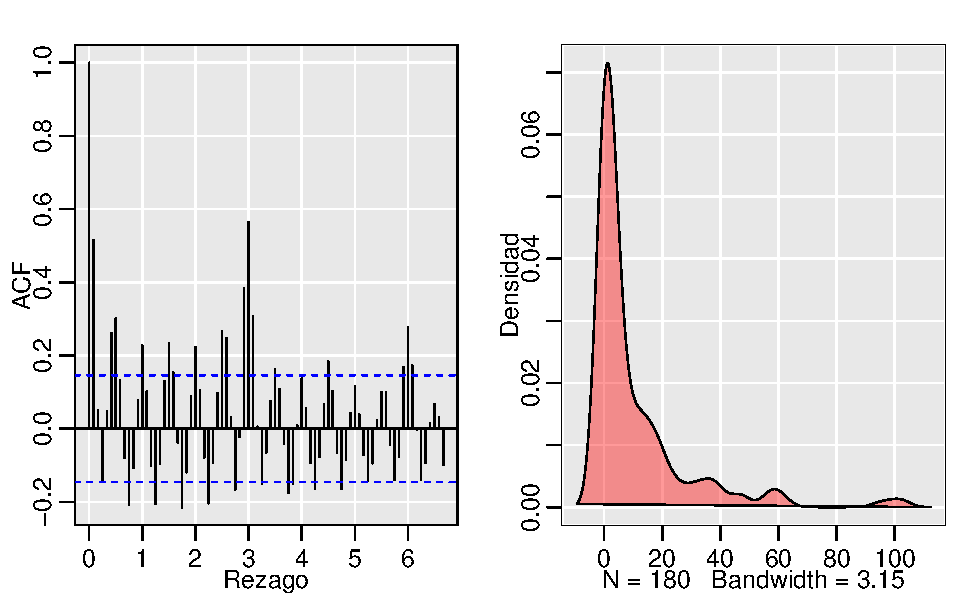
\includegraphics[width=\maxwidth]{figure/unnamed-chunk-38-1} \caption[Función de autocorrelación muetral, para la serie GIF]{Función de autocorrelación muetral, para la serie GIF.}\label{fig:unnamed-chunk-38}
\end{figure}


\end{knitrout}


Como se vio en la tabla 11 y 12, a
\section{Anexo Códigos}

\begin{knitrout}
\definecolor{shadecolor}{rgb}{0.91, 0.91, 0.91}\color{fgcolor}\begin{kframe}
\begin{alltt}
\hlcom{################ Packages ###}
\hlkwd{library}\hlstd{(Bayeshmmcts)}
\hlkwd{library}\hlstd{(broom)}


\hlcom{################ Data #####}
\hlkwd{data}\hlstd{(}\hlstr{"homicidios"}\hlstd{)}
\hlkwd{data}\hlstd{(}\hlstr{"incendios"}\hlstd{)}

\hlcom{################################################### Poisson - Hidden Markov Model ##########}


\hlkwd{rm}\hlstd{(}\hlkwc{list} \hlstd{=} \hlkwd{ls}\hlstd{())}

\hlcom{################################################### Zero Inflated Poisson - Hidden Markov Model ###}

\hlstd{incendios} \hlkwb{<-} \hlkwd{readRDS}\hlstd{(}\hlstr{"incendios.rds"}\hlstd{)}
\hlstd{GIF} \hlkwb{<-} \hlkwd{ts}\hlstd{(}\hlkwc{data} \hlstd{= incendios}\hlopt{$}\hlstd{GIF,} \hlkwc{start} \hlstd{=} \hlkwd{c}\hlstd{(}\hlnum{2002}\hlstd{,} \hlnum{1}\hlstd{),} \hlkwc{frequency} \hlstd{=} \hlnum{12}\hlstd{)}
\hlstd{GIF}
\end{alltt}
\end{kframe}
\end{knitrout}



\end{document}
